% Options for packages loaded elsewhere
\PassOptionsToPackage{unicode}{hyperref}
\PassOptionsToPackage{hyphens}{url}
\PassOptionsToPackage{dvipsnames,svgnames,x11names}{xcolor}
%
\documentclass[
  super,
  preprint,
  3p]{elsarticle}

\usepackage{amsmath,amssymb}
\usepackage{lmodern}
\usepackage{iftex}
\ifPDFTeX
  \usepackage[T1]{fontenc}
  \usepackage[utf8]{inputenc}
  \usepackage{textcomp} % provide euro and other symbols
\else % if luatex or xetex
  \usepackage{unicode-math}
  \defaultfontfeatures{Scale=MatchLowercase}
  \defaultfontfeatures[\rmfamily]{Ligatures=TeX,Scale=1}
\fi
% Use upquote if available, for straight quotes in verbatim environments
\IfFileExists{upquote.sty}{\usepackage{upquote}}{}
\IfFileExists{microtype.sty}{% use microtype if available
  \usepackage[]{microtype}
  \UseMicrotypeSet[protrusion]{basicmath} % disable protrusion for tt fonts
}{}
\makeatletter
\@ifundefined{KOMAClassName}{% if non-KOMA class
  \IfFileExists{parskip.sty}{%
    \usepackage{parskip}
  }{% else
    \setlength{\parindent}{0pt}
    \setlength{\parskip}{6pt plus 2pt minus 1pt}}
}{% if KOMA class
  \KOMAoptions{parskip=half}}
\makeatother
\usepackage{xcolor}
\setlength{\emergencystretch}{3em} % prevent overfull lines
\setcounter{secnumdepth}{5}
% Make \paragraph and \subparagraph free-standing
\ifx\paragraph\undefined\else
  \let\oldparagraph\paragraph
  \renewcommand{\paragraph}[1]{\oldparagraph{#1}\mbox{}}
\fi
\ifx\subparagraph\undefined\else
  \let\oldsubparagraph\subparagraph
  \renewcommand{\subparagraph}[1]{\oldsubparagraph{#1}\mbox{}}
\fi


\providecommand{\tightlist}{%
  \setlength{\itemsep}{0pt}\setlength{\parskip}{0pt}}\usepackage{longtable,booktabs,array}
\usepackage{calc} % for calculating minipage widths
% Correct order of tables after \paragraph or \subparagraph
\usepackage{etoolbox}
\makeatletter
\patchcmd\longtable{\par}{\if@noskipsec\mbox{}\fi\par}{}{}
\makeatother
% Allow footnotes in longtable head/foot
\IfFileExists{footnotehyper.sty}{\usepackage{footnotehyper}}{\usepackage{footnote}}
\makesavenoteenv{longtable}
\usepackage{graphicx}
\makeatletter
\def\maxwidth{\ifdim\Gin@nat@width>\linewidth\linewidth\else\Gin@nat@width\fi}
\def\maxheight{\ifdim\Gin@nat@height>\textheight\textheight\else\Gin@nat@height\fi}
\makeatother
% Scale images if necessary, so that they will not overflow the page
% margins by default, and it is still possible to overwrite the defaults
% using explicit options in \includegraphics[width, height, ...]{}
\setkeys{Gin}{width=\maxwidth,height=\maxheight,keepaspectratio}
% Set default figure placement to htbp
\makeatletter
\def\fps@figure{htbp}
\makeatother

\usepackage{amsmath}
\usepackage{booktabs}
\usepackage{caption}
\usepackage{longtable}
\makeatletter
\makeatother
\makeatletter
\makeatother
\makeatletter
\@ifpackageloaded{caption}{}{\usepackage{caption}}
\AtBeginDocument{%
\ifdefined\contentsname
  \renewcommand*\contentsname{Table of contents}
\else
  \newcommand\contentsname{Table of contents}
\fi
\ifdefined\listfigurename
  \renewcommand*\listfigurename{List of Figures}
\else
  \newcommand\listfigurename{List of Figures}
\fi
\ifdefined\listtablename
  \renewcommand*\listtablename{List of Tables}
\else
  \newcommand\listtablename{List of Tables}
\fi
\ifdefined\figurename
  \renewcommand*\figurename{Figure}
\else
  \newcommand\figurename{Figure}
\fi
\ifdefined\tablename
  \renewcommand*\tablename{Table}
\else
  \newcommand\tablename{Table}
\fi
}
\@ifpackageloaded{float}{}{\usepackage{float}}
\floatstyle{ruled}
\@ifundefined{c@chapter}{\newfloat{codelisting}{h}{lop}}{\newfloat{codelisting}{h}{lop}[chapter]}
\floatname{codelisting}{Listing}
\newcommand*\listoflistings{\listof{codelisting}{List of Listings}}
\makeatother
\makeatletter
\@ifpackageloaded{caption}{}{\usepackage{caption}}
\@ifpackageloaded{subcaption}{}{\usepackage{subcaption}}
\makeatother
\makeatletter
\@ifpackageloaded{tcolorbox}{}{\usepackage[many]{tcolorbox}}
\makeatother
\makeatletter
\@ifundefined{shadecolor}{\definecolor{shadecolor}{rgb}{.97, .97, .97}}
\makeatother
\makeatletter
\makeatother
\journal{To be determined}
\ifLuaTeX
  \usepackage{selnolig}  % disable illegal ligatures
\fi
\usepackage[]{natbib}
\bibliographystyle{elsarticle-num}
\IfFileExists{bookmark.sty}{\usepackage{bookmark}}{\usepackage{hyperref}}
\IfFileExists{xurl.sty}{\usepackage{xurl}}{} % add URL line breaks if available
\urlstyle{same} % disable monospaced font for URLs
\hypersetup{
  pdftitle={Extracorporeal CPR for Refractory Out-of-Hospital Cardiac Arrest},
  pdfauthor={James M Brophy},
  pdfkeywords={extracorporeal CPR, Bayesian statistics},
  colorlinks=true,
  linkcolor={blue},
  filecolor={Maroon},
  citecolor={Blue},
  urlcolor={Blue},
  pdfcreator={LaTeX via pandoc}}

\setlength{\parindent}{6pt}
\begin{document}

\begin{frontmatter}
\title{Extracorporeal CPR for Refractory Out-of-Hospital Cardiac
Arrest \\\large{A Bayesian Perspective} }
\author[1]{James M Brophy%
\corref{cor1}%
\fnref{fn1}}
 \ead{james.brophy@mcgill.ca} 

\affiliation[1]{organization={McGill University Health Center, Centre
for Health Outcomes Research (CORE)},addressline={5252 Boul. de
Maisonneuve West Room 2B.37},city={Montreal},postcode={H4A
3S5},postcodesep={}}

\cortext[cor1]{Corresponding author}
\fntext[fn1]{JMB is a research scholar supported by Les Fonds de
Recherche Québec Santé}
        
\begin{abstract}
A recent randomized clinical trial reported in patients with refractory
out-of-hospital cardiac arrest, extracorporeal CPR and conventional CPR
had similar effects on survival with a favorable neurologic outcome.
Herein, it is examined whether a Bayesian perspective allows any
additional insights into the interpretation of this trial.
\end{abstract}





\begin{keyword}
    extracorporeal CPR \sep 
    Bayesian statistics
\end{keyword}
\end{frontmatter}
    \ifdefined\Shaded\renewenvironment{Shaded}{\begin{tcolorbox}[boxrule=0pt, borderline west={3pt}{0pt}{shadecolor}, sharp corners, breakable, interior hidden, enhanced, frame hidden]}{\end{tcolorbox}}\fi

\hypertarget{introduction}{%
\section{Introduction}\label{introduction}}

Out-of-hospital cardiac arrest is a frequent event and fortunately its
devastating consequences can be partially mitigated by rapid
commencement of basic life support with high-quality chest compressions
and external defibrillation (conventional cardiopulmonary resuscitation
(CPR)). However, there remains a substantial subset of individuals who
do not respond rapidly to these measures and whether more invasive
measures. Whether the addition of more aggressive measure including
extracorporeal CPR (the addition of extracorporeal membrane oxygenation
to standard advanced cardiac life support (eCPR)) can improve survival
and diminish anoxic brain injury is a current topic of research. The
largest randomized clinical trial (RCT) examining this question recently
published their results\citep{CPR2023a}. For the primary outcome, 30 day
survival without significant neurological deficit, the authors observed
an odds ratio of 1.4 (95\% confidence interval, 0.5 to 3.5; P = 0.52) in
favor of extracorporeal CPR for leading to their conclusion ``In
patients with refractory out-of-hospital cardiac arrest, extracorporeal
CPR and conventional CPR had similar effects on survival with a
favorable neurological outcome''.\citep{CPR2023a}

This communication does not reiterate the many reasons to be wary of
null hypothesis significance testing (NHST), p values and confidence
intervals\citep{RN5420}. Rather it assumes the reader has perhaps heard
that Bayesian methods mirror our intuitive learning process and is
curious about its potential application to RCT interpretations.

Therefore the goal of this communication is to examine whether a
Bayesian perspective permits additional insights into the specific
clinical question regarding any added value of extracorporeal CPR
following an out-of-hospital arrest in patients refractory to standard
CPR.

\hypertarget{methods}{%
\section{Methods}\label{methods}}

The data for the primary outcome, 30 day survival with intact
neurological status, based on an intention to treat (ITT) analysis was
abstracted from the original INCEPTION trial \citep{CPR2023a} and used
for the primary analysis. The ITT analysis has the advantage of
minimizing bias by preserving the prognostic balance afforded by
randomization as well as assuring the validity of the statistical
analyses.

Bayesian analytical approaches provide a number of benefits over the
classical NHST approach, including parameter estimation accompanied by
direct probability statements about parameters of interest (herein the
risk of survival with intact neurological status), and the incorporation
prior knowledge \citep{BrophyCardio, Zampieri}.

These probability statements arise from the posterior distribution
according to the following equation:
\[ \text{Posterior}  = \frac{\text{Probability of the data} * \text{Prior}}{\text{Normalizing Constant}} \]

Therefore, in addition to the current data summarized by the probability
of the data (likelihood function) one requires a prior probability
distribution for each parameter. The mechanics of the Bayesian analyses
were performed using the Stan programming language \citep{stan} through
the R package rstanarm \citep{rstanarm} and fit a logistic regression
model with a single treatment parameter, \(\theta\). Because our focus
is the interpretation of the INCEPTION trial alone, our primary analysis
used rstanarm's default vague parameter priors
(\(log(\theta) \sim Normal [0, 2.50]\), thereby assuring that the
posterior distribution is dominated by the observed INCEPTION data.

The robustness of the Bayesian approach is often assessed by sensitivity
analyses that examine the variation in the posterior probability as a
function of the choice of different prior distributions. Using prior
information also underscores the important advantage of Bayesian
analyses to learn sequentially. There were two previous RCTs examining
extracorporeal CPR\citep{RN6759, RN6751} and while the protocols are not
identical, it may be reasonable to allow this data to serve as informed
priors for the eCPR parameter, which can be updated with the INCEPTION
data.

This prior information of the probability of eCPR success in each
previous trial, \(X_i\), can be summarized as a normal distribution with
a mean equal to the proportion of successes, \(\hat{p_i}\) with a
standard deviation equal to \[\sqrt{\hat{p_i}*(1-\hat{p_i})}\] As
baseline success rates for standard CPR varies markedly between the
three studies, it was decided to maintain the INCEPTION control baseline
with the vague prior for all analyses and to update only the eCPR arm
with prior information.

Posterior distributions are summarized with medians and 95\%
highest-density intervals (credible intervals), defined as the narrowest
interval containing 95\% of the probability density function
\citep{mcelreath2020}. We not only calculated the posterior probability
of any additional survival with eCPR (OR \textgreater1.00), but also of
clinically meaningful benefits (defined as OR \textgreater1.10).

ITT assesses subjects based on the group they were initially (and
randomly) allocated to, regardless of whether or not they dropped out,
were fully adhered to the treatment or switched to an alternative
treatment. ITT analyses can therefore be seen as a conservative estimate
which mirrors clinical effectiveness. In contrast, a per protocol (PP)
analysis involves a comparison of treatment groups in a trial that
includes only those patients who completed the treatment they were
originally allocated to. Similarly an ``as treated'' analysis considers
only which treatments subjects received, regardless of their
randomization status and protocol adherence. While both PP and
as-treated analyses alone may lead to bias, in conjunction with an ITT
analysis they may provide additional insights into efficacy and have
also been examined from a Bayesian perspective.

All analyses were executed using \texttt{R}\citep{R} within the
integrated development environment of RStudio. Bayesian analyses were
performed using the front end \texttt{rstanarm} package\citep{rstanarm}
to the \texttt{Stan} programming language{[}stan{]}. The statistical
code can be found on Github (https://github.com/brophyj/eCPR).

\hypertarget{results}{%
\section{Results}\label{results}}

ITT data from the INCEPTION trial\citep{CPR2023a} and two other
pertinent trials\citep{RN6751, RN6759} that also randomized CPR to eCPR
are shown in Table 1. Performing a Bayesian analysis on the INCEPTION
trial, using the default vague prior, produces an odds ratio (OR) 1.32
(95\% Credible Interval (CrI) 0.54 - 3.22). The closeness of this result
to the original analysis (OR, 1.4; 95\% CI 0.5 - 3.5) confirms no impact
of the vague prior and shows this Bayesian analysis is completely
dominated by the observed INCEPTION data.

One of the advantages of a Bayesian approach is the ability to make
direct probability statements about the estimand of improved survival
with eCPR. The eCPR probability density function for improved survival
from INCEPTION data with the default vague prior is displayed in Figure
1 and reveals that the probability of enhanced survival with eCPR is
72.72\%. The probability that the improved survival exceeds a 10\%
improvement is 0.66\%.

Another advantage of a Bayesian approach is the possibility of including
previous evidence as informed priors. We considered three possible
scenarios i) using all the available prior RCT
data\citep{RN6751, RN6759} to create a combined prior which was
expressed as a N(0.32, 0.47)\\
ii) using only the ARREST data, labelled an enthusiastic prior, as this
trial was stopped prematurely for efficacy, expressed as a N(0.43,
0.49)\\
iii) using only the PRAGUE data, labelled a skeptical prior, as this
trial was stopped prematurely for futility, expressed as a N(0.31, 0.46)

These different prior probabilities can be updated using the INCEPTION
to create posterior distributions that are summarized in Table 2.
Basically, it is observed that in all cases the point estimate for the
enhanced eCPR survival remains fairly constant but the associated
uncertainty is reduced with the additional data as reflected by the
narrower 95\% CrI. The posterior probability of improved eCPR survival
goes from 80\% with a skeptical prior to 85\% with the enthusiastic
prior.

\newpage

\hypertarget{tables}{%
\section{Tables}\label{tables}}

\setlength{\LTpost}{0mm}
\begin{longtable}{lcccc}
\caption*{
{\large Table 1 Extracted ITT trial data}
} \\ 
\toprule
Trial & Fail CPR (n) & Fail eCPR (n) & Success CPR (n) & Success eCPR (n) \\ 
\midrule
INCEPTION & 52 & 56 & 10 & 14 \\ 
ARREST & 15 & 8 & 0 & 6 \\ 
PRAGUE & 108 & 86 & 24 & 38 \\ 
\bottomrule
\end{longtable}
\begin{minipage}{\linewidth}
eCPR = extracorporeal cardiopulmonary resuscitation\\
\end{minipage}

\setlength{\LTpost}{0mm}
\begin{longtable}{lcccc}
\caption*{
{\large Table 2 Probabilities of improved survival with eCPR with various priors}
} \\ 
\toprule
Priors & OR & \multicolumn{2}{c}{95\% CrI} & Probability \\ 
\cmidrule(lr){1-1} \cmidrule(lr){2-2} \cmidrule(lr){3-4} \cmidrule(lr){5-5}
 & point estimate & lower limit & upper limit & p(OR) >1  \\ 
\midrule
Vague & 1.32 & 0.543 & 3.21 & 0.727 \\ 
Combined & 1.35 & 0.705 & 2.58 & 0.817 \\ 
Enthusiastic & 1.40 & 0.738 & 2.67 & 0.849 \\ 
Skeptical & 1.32 & 0.700 & 2.50 & 0.804 \\ 
\bottomrule
\end{longtable}
\begin{minipage}{\linewidth}
Vague: default vague prior\\
Combined: prior eCPR data from ARREST + PRAGUE\\
Enthusiastic: prior eCPR data from ARREST alone\\
Skeptical: prior eCPR data from PRAGUE alone\\
\end{minipage}

\newpage

\hypertarget{figures}{%
\section{Figures}\label{figures}}

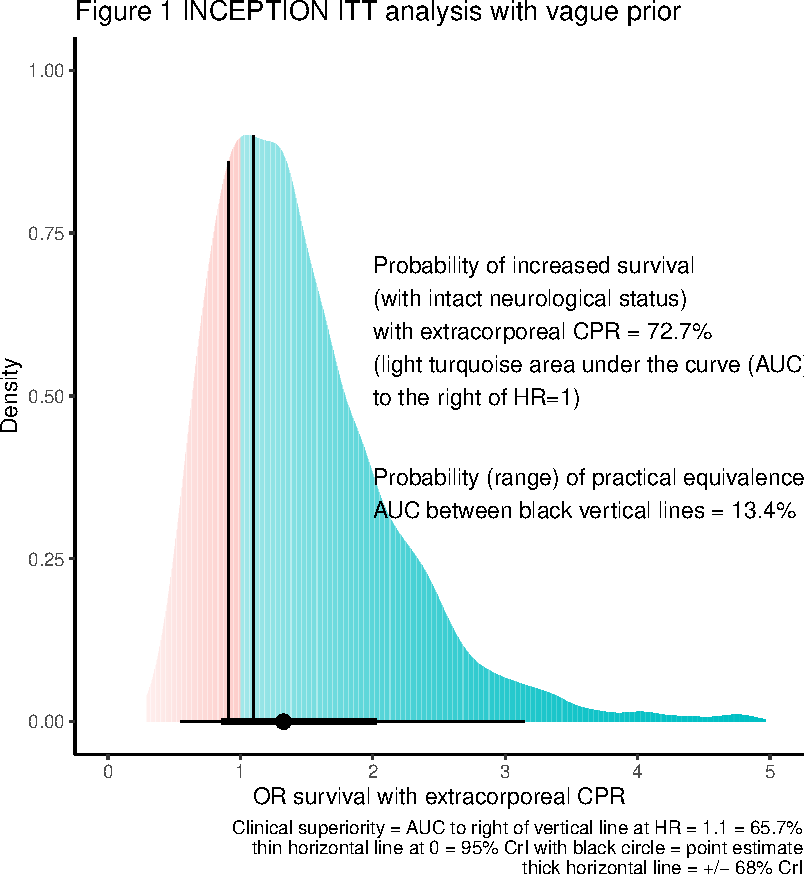
\includegraphics{manuscript_files/figure-pdf/fig1-1.pdf}

\newpage

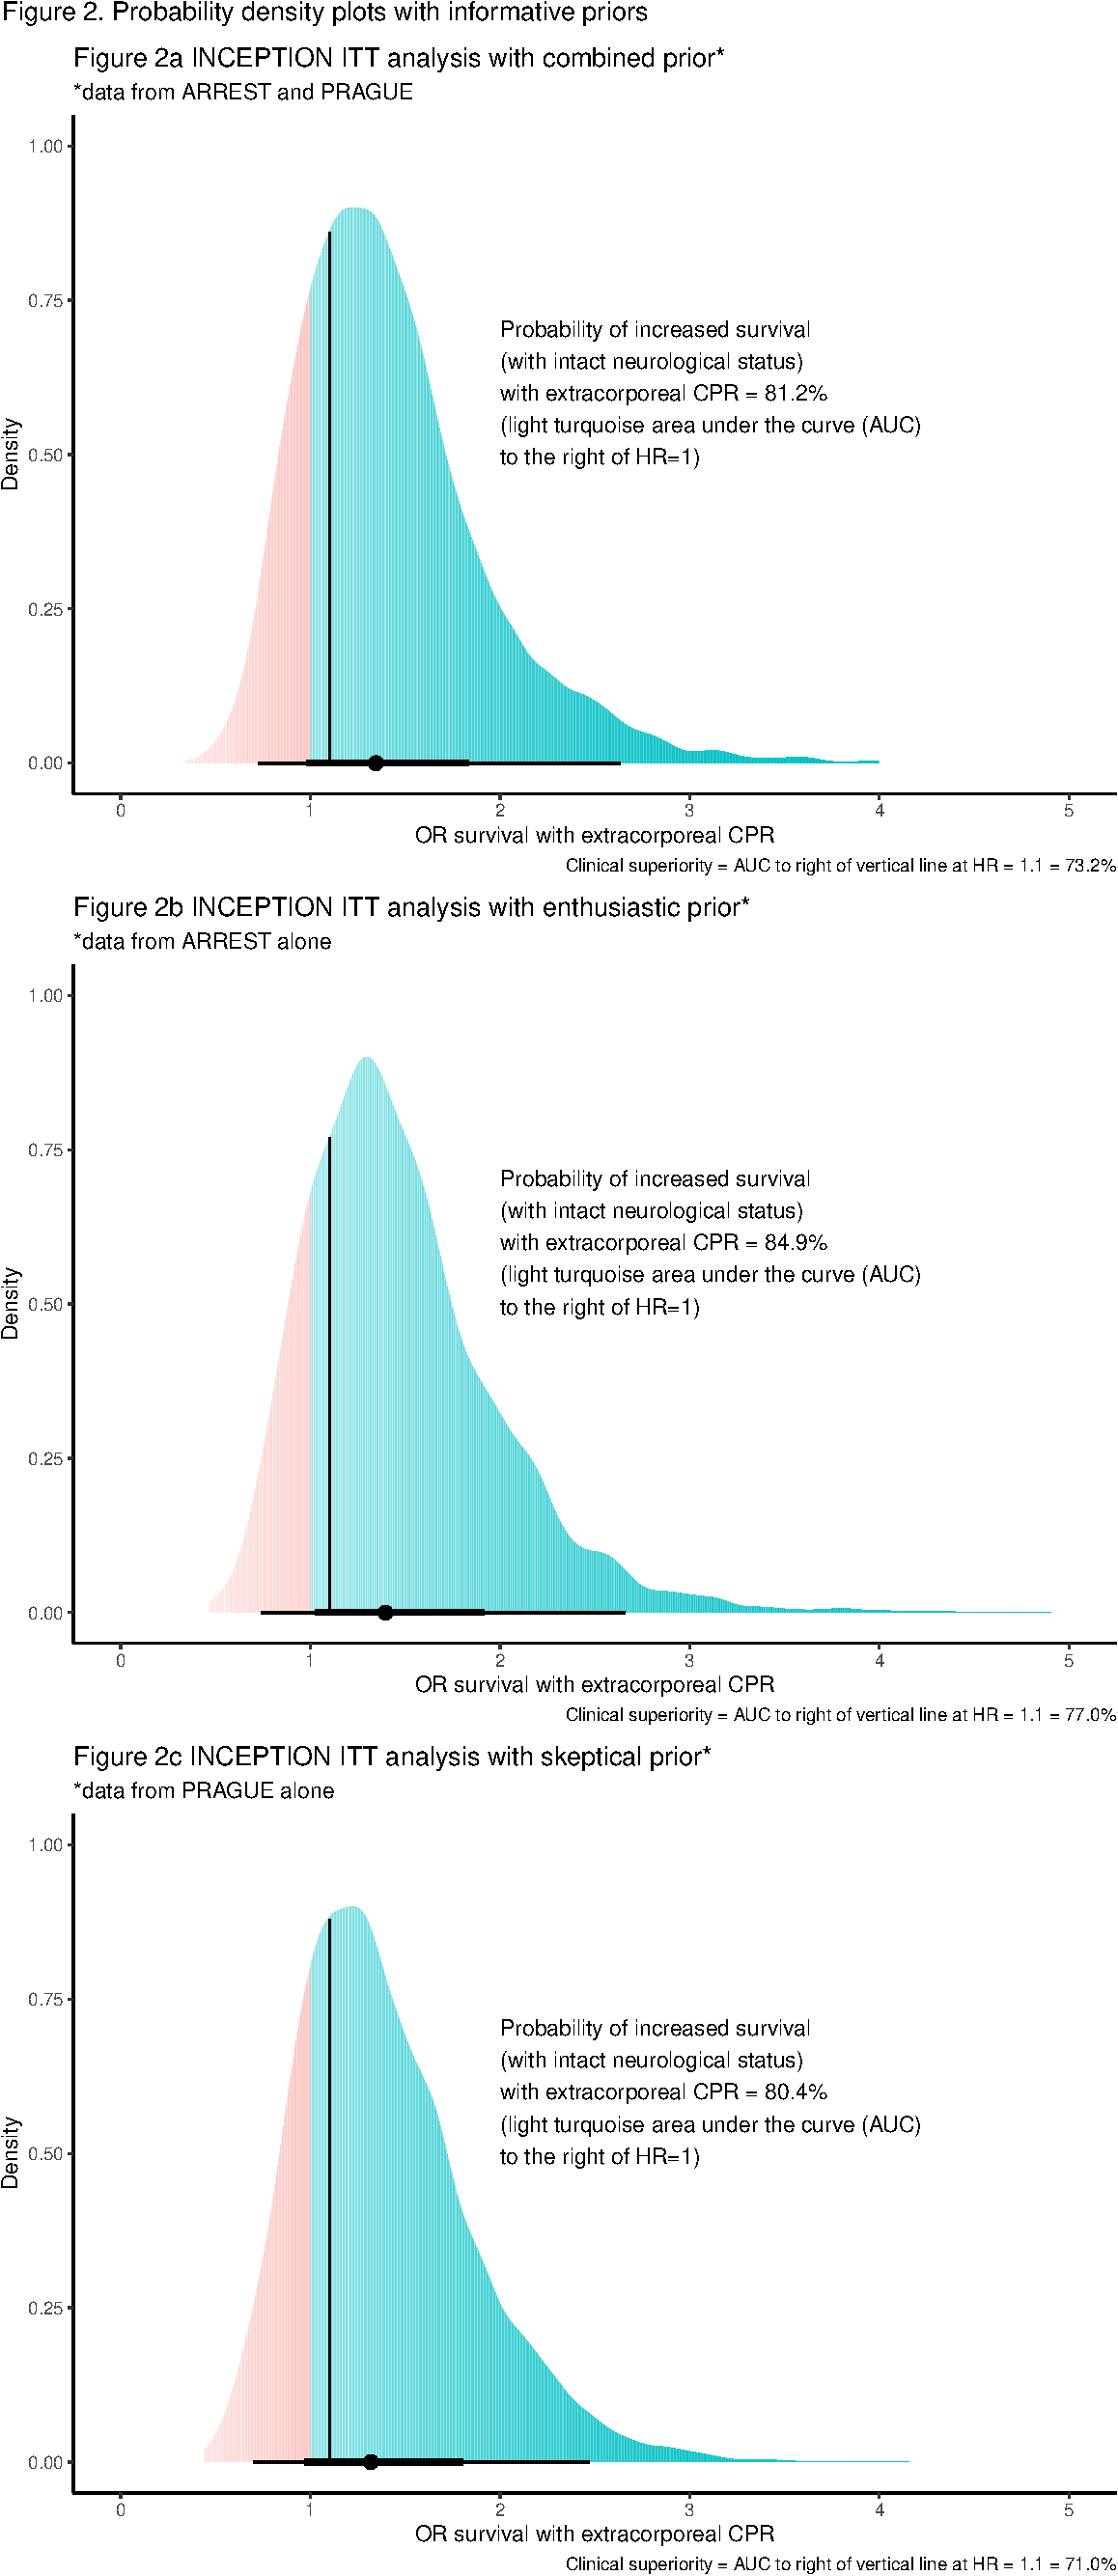
\includegraphics{manuscript_files/figure-pdf/fig2-1.pdf}

\newpage


\renewcommand\refname{References}
  \bibliography{bibliography.bib}


\end{document}
